% Created by tikzDevice version 0.10.1 on 2017-06-15 12:55:53
% !TEX encoding = UTF-8 Unicode
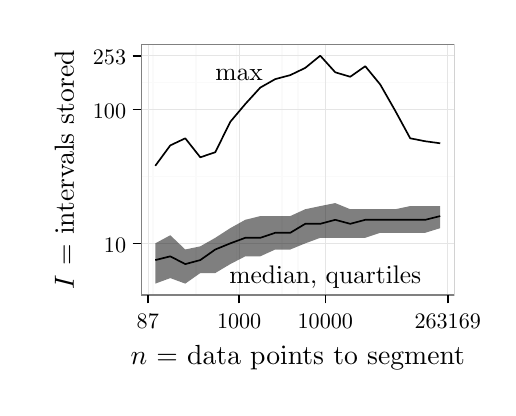
\begin{tikzpicture}[x=1pt,y=1pt]
\definecolor{fillColor}{RGB}{255,255,255}
\path[use as bounding box,fill=fillColor,fill opacity=0.00] (0,0) rectangle (166.22,130.09);
\begin{scope}
\path[clip] (  0.00,  0.00) rectangle (166.22,130.09);
\definecolor{drawColor}{RGB}{255,255,255}
\definecolor{fillColor}{RGB}{255,255,255}

\path[draw=drawColor,line width= 0.6pt,line join=round,line cap=round,fill=fillColor] (  0.00,  0.00) rectangle (166.22,130.09);
\end{scope}
\begin{scope}
\path[clip] ( 40.96, 33.48) rectangle (154.22,124.09);
\definecolor{fillColor}{RGB}{255,255,255}

\path[fill=fillColor] ( 40.96, 33.48) rectangle (154.22,124.09);
\definecolor{drawColor}{gray}{0.98}

\path[draw=drawColor,line width= 0.6pt,line join=round] ( 40.96, 76.31) --
	(154.22, 76.31);

\path[draw=drawColor,line width= 0.6pt,line join=round] ( 40.96,110.22) --
	(154.22,110.22);

\path[draw=drawColor,line width= 0.6pt,line join=round] ( 45.28, 33.48) --
	( 45.28,124.09);

\path[draw=drawColor,line width= 0.6pt,line join=round] ( 60.85, 33.48) --
	( 60.85,124.09);

\path[draw=drawColor,line width= 0.6pt,line join=round] ( 91.99, 33.48) --
	( 91.99,124.09);

\path[draw=drawColor,line width= 0.6pt,line join=round] ( 75.48, 33.48) --
	( 75.48,124.09);

\path[draw=drawColor,line width= 0.6pt,line join=round] ( 97.59, 33.48) --
	( 97.59,124.09);
\definecolor{drawColor}{gray}{0.90}

\path[draw=drawColor,line width= 0.2pt,line join=round] ( 40.96, 52.15) --
	(154.22, 52.15);

\path[draw=drawColor,line width= 0.2pt,line join=round] ( 40.96,100.48) --
	(154.22,100.48);

\path[draw=drawColor,line width= 0.2pt,line join=round] ( 40.96,119.97) --
	(154.22,119.97);

\path[draw=drawColor,line width= 0.2pt,line join=round] ( 76.42, 33.48) --
	( 76.42,124.09);

\path[draw=drawColor,line width= 0.2pt,line join=round] (107.56, 33.48) --
	(107.56,124.09);

\path[draw=drawColor,line width= 0.2pt,line join=round] ( 43.40, 33.48) --
	( 43.40,124.09);

\path[draw=drawColor,line width= 0.2pt,line join=round] (151.78, 33.48) --
	(151.78,124.09);
\definecolor{drawColor}{RGB}{0,0,0}

\node[text=drawColor,anchor=base,inner sep=0pt, outer sep=0pt, scale=  0.92] at ( 76.42,111.18) {max};

\node[text=drawColor,anchor=base,inner sep=0pt, outer sep=0pt, scale=  0.92] at (107.56, 37.62) {median, quartiles};

\path[draw=drawColor,line width= 0.6pt,line join=round] ( 46.11, 80.17) --
	( 51.53, 87.55) --
	( 56.95, 90.11) --
	( 62.37, 83.25) --
	( 67.79, 85.07) --
	( 73.21, 96.06) --
	( 78.62,102.48) --
	( 84.04,108.43) --
	( 89.46,111.50) --
	( 94.88,112.94) --
	(100.30,115.55) --
	(105.72,119.97) --
	(111.14,113.96) --
	(116.56,112.35) --
	(121.98,116.16) --
	(127.40,109.55) --
	(132.82,100.06) --
	(138.23, 90.11) --
	(143.65, 89.05) --
	(149.07, 88.31);
\definecolor{fillColor}{RGB}{0,0,0}

\path[fill=fillColor,fill opacity=0.50] ( 46.11, 52.15) --
	( 51.53, 55.08) --
	( 56.95, 49.93) --
	( 62.37, 51.07) --
	( 67.79, 54.15) --
	( 73.21, 57.65) --
	( 78.62, 60.66) --
	( 84.04, 62.01) --
	( 89.46, 62.01) --
	( 94.88, 62.01) --
	(100.30, 64.48) --
	(105.72, 65.62) --
	(111.14, 66.70) --
	(116.56, 64.48) --
	(121.98, 64.48) --
	(127.40, 64.48) --
	(132.82, 64.48) --
	(138.23, 65.62) --
	(143.65, 65.62) --
	(149.07, 65.62) --
	(149.07, 57.65) --
	(143.65, 55.97) --
	(138.23, 55.97) --
	(132.82, 55.97) --
	(127.40, 55.97) --
	(121.98, 54.15) --
	(116.56, 54.15) --
	(111.14, 54.15) --
	(105.72, 54.15) --
	(100.30, 52.15) --
	( 94.88, 49.93) --
	( 89.46, 49.93) --
	( 84.04, 47.46) --
	( 78.62, 47.46) --
	( 73.21, 44.66) --
	( 67.79, 41.42) --
	( 62.37, 41.42) --
	( 56.95, 37.60) --
	( 51.53, 39.60) --
	( 46.11, 37.60) --
	cycle;

\path[draw=drawColor,line width= 0.6pt,line join=round] ( 46.11, 46.11) --
	( 51.53, 47.46) --
	( 56.95, 44.66) --
	( 62.37, 46.11) --
	( 67.79, 49.93) --
	( 73.21, 52.15) --
	( 78.62, 54.15) --
	( 84.04, 54.15) --
	( 89.46, 55.97) --
	( 94.88, 55.97) --
	(100.30, 59.21) --
	(105.72, 59.21) --
	(111.14, 60.66) --
	(116.56, 59.21) --
	(121.98, 60.66) --
	(127.40, 60.66) --
	(132.82, 60.66) --
	(138.23, 60.66) --
	(143.65, 60.66) --
	(149.07, 62.01);
\definecolor{drawColor}{gray}{0.50}

\path[draw=drawColor,line width= 0.6pt,line join=round,line cap=round] ( 40.96, 33.48) rectangle (154.22,124.09);
\end{scope}
\begin{scope}
\path[clip] (  0.00,  0.00) rectangle (166.22,130.09);
\definecolor{drawColor}{RGB}{0,0,0}

\node[text=drawColor,anchor=base east,inner sep=0pt, outer sep=0pt, scale=  0.80] at ( 35.56, 48.84) {10};

\node[text=drawColor,anchor=base east,inner sep=0pt, outer sep=0pt, scale=  0.80] at ( 35.56, 97.18) {100};

\node[text=drawColor,anchor=base east,inner sep=0pt, outer sep=0pt, scale=  0.80] at ( 35.56,116.66) {253};
\end{scope}
\begin{scope}
\path[clip] (  0.00,  0.00) rectangle (166.22,130.09);
\definecolor{drawColor}{RGB}{0,0,0}

\path[draw=drawColor,line width= 0.6pt,line join=round] ( 37.96, 52.15) --
	( 40.96, 52.15);

\path[draw=drawColor,line width= 0.6pt,line join=round] ( 37.96,100.48) --
	( 40.96,100.48);

\path[draw=drawColor,line width= 0.6pt,line join=round] ( 37.96,119.97) --
	( 40.96,119.97);
\end{scope}
\begin{scope}
\path[clip] (  0.00,  0.00) rectangle (166.22,130.09);
\definecolor{drawColor}{RGB}{0,0,0}

\path[draw=drawColor,line width= 0.6pt,line join=round] ( 76.42, 30.48) --
	( 76.42, 33.48);

\path[draw=drawColor,line width= 0.6pt,line join=round] (107.56, 30.48) --
	(107.56, 33.48);

\path[draw=drawColor,line width= 0.6pt,line join=round] ( 43.40, 30.48) --
	( 43.40, 33.48);

\path[draw=drawColor,line width= 0.6pt,line join=round] (151.78, 30.48) --
	(151.78, 33.48);
\end{scope}
\begin{scope}
\path[clip] (  0.00,  0.00) rectangle (166.22,130.09);
\definecolor{drawColor}{RGB}{0,0,0}

\node[text=drawColor,anchor=base,inner sep=0pt, outer sep=0pt, scale=  0.80] at ( 76.42, 21.46) {1000};

\node[text=drawColor,anchor=base,inner sep=0pt, outer sep=0pt, scale=  0.80] at (107.56, 21.46) {10000};

\node[text=drawColor,anchor=base,inner sep=0pt, outer sep=0pt, scale=  0.80] at ( 43.40, 21.46) {87};

\node[text=drawColor,anchor=base,inner sep=0pt, outer sep=0pt, scale=  0.80] at (151.78, 21.46) {263169};
\end{scope}
\begin{scope}
\path[clip] (  0.00,  0.00) rectangle (166.22,130.09);
\definecolor{drawColor}{RGB}{0,0,0}

\node[text=drawColor,anchor=base,inner sep=0pt, outer sep=0pt, scale=  1.00] at ( 97.59,  8.40) {$n$ = data points to segment};
\end{scope}
\begin{scope}
\path[clip] (  0.00,  0.00) rectangle (166.22,130.09);
\definecolor{drawColor}{RGB}{0,0,0}

\node[text=drawColor,rotate= 90.00,anchor=base,inner sep=0pt, outer sep=0pt, scale=  1.00] at ( 16.66, 78.78) {$I$ = intervals stored};
\end{scope}
\end{tikzpicture}
